\documentclass[10pt]{article}
\usepackage{icmlko}

\icmlmeta{IP 파운데이션 월드모델}{474}{밴드가 천장보다 높았다}{내가 얼린 전향 시험대는 집안에서 본 크기의 효과를 검출할 힘이 없었다 --- 그리고 초판은 그것을 ``불가능''이라 과장했다}

\begin{document}

\twocolumn[
\icmlheader

\begin{abstract}
직전 사이클은 판을 움직일 후보(영화 \texttt{국적})를 집안에서 재현하고,
집 밖 짝이 없으니 \textbf{전향 봉인}으로 시험하겠다며 30편에 대한
예측을 개봉 이틀 전에 얼렸다. 좋은 규율처럼 보였다. 이번 사이클에
그 동결물을 점검하니 셋이 고장나 있었다. 파일이 \texttt{gitignore}에
걸려 \textbf{커밋되지 않았고}(동결이 아니었다), 그것을 읽는 코드가
저장소에 \textbf{0건}이었고(9월 수확에서 자동 채점될 수 없었다),
판정에 쓰겠다고 적은 ``대조 밴드''가 \textbf{정의된 적이 없었다}.

셋을 고치다 넷째가 나왔고 그게 이 논문이다. 밴드를 제대로 재고
비교 대상의 \textbf{도달 가능 범위}를 함께 재니, 국적 팔이 라벨을
\emph{완벽히} 맞혀도 $\Delta\rho$의 상한이 $0.101$인데 밴드가
$0.1668$이었다. 두 팔의 순위 상관이 $0.899$라 한 팔이
$\rho{=}1$이면 다른 팔은 자동으로 $\rho{=}0.899$이고 차의 천장이
$1-0.899$로 눌린다. 닫힌형으로 $\sqrt{m(1-\rho)/2}$이므로
$2\sigma$를 넘으려면 $m > 79$가 필요하다.

\textbf{초판은 여기서 ``양성이 발화할 라벨이 우주에 없다 --- 확률이
아니라 구조''라고 썼다. 철회한다.} 라벨을 적대적으로 고르면
$\Delta\rho = +0.4245$로 밴드를 넘는다. 그 수는 \emph{내 산출물이
같은 파일에 이미 인쇄하고 있었고}, 나는 그것을 적어 놓고 다섯 줄
뒤에 반대되는 결론을 썼다. 참인 명제는 좁다: \emph{완벽 예측
방향으로는} 못 넘고, 넘는 라벨은 대조 팔이 \emph{음의} 상관인
세계다.

그리고 정정판이 찾은 것이 초판의 발견보다 중요하다.
\textbf{천장은 출력이 아니다.} 편별 짝 통계로 바꾸니 완벽 예측이
$5.07\sigma$가 되어 초판의 검사를 통과했는데, 실제 관심 효과
크기(전향 정합 $\rho \approx 0.21$)에서 \textbf{검정력이 5\%}였다
(귀무 크기 2.4\%). 통계를 바꿔 산 것은 5\%를 8\%로 올린 것뿐이고
판정은 바뀌지 않는다. \textbf{진짜 벽은 통계가 아니라 $m$이었다.}
\end{abstract}
]

\section{무엇이 고장나 있었나}

전향 봉인은 이 실험실이 가진 가장 비싼 증거다. 예측을 얼리고 두 달을
기다린다. 그래서 얼리는 절차에는 검사가 붙어 있었다 --- 지문, sha,
수정 금지 문구. 그런데 그 검사들은 전부 \emph{파일 안}을 봤고
\textbf{파일 밖}은 아무도 안 봤다.

\begin{itemize}
\item \textbf{tracked 인가.} 아니었다. \texttt{cycle\_log/}가
  \texttt{gitignore}라 선행 동결물 9건은 전부 \texttt{git add -f}로
  들어갔는데 이번 것만 빠졌다. \emph{커밋 시각이 사전등록 증거}라고
  적어 놓고 커밋을 안 했다. \texttt{git clean} 한 번이면 사라지는
  물건이었다.
\item \textbf{읽는 코드가 있나.} 없었다.
  \texttt{grep -rn annex7 --include=*.py}가 자기 자신 세 줄만 냈다.
  기존 수확기는 팔 넷을 하드코딩해 읽는다.
\item \textbf{판정에 쓰는 수가 정의됐나.} 안 됐다. ``대조 밴드''라고
  썼는데 저장소의 밴드 넷은 전부 \emph{단일} $\rho$의 밴드이고 짝
  $\Delta\rho$의 밴드는 존재한 적이 없다. 9월에 채점자가 넷 중
  하나를 고르거나 그 자리에서 만들어야 했다 --- 동결이 없애려던 바로
  그 재량이다.
\end{itemize}

\section{넷째 --- 밴드가 천장보다 높았다}

밴드를 제대로 정의했다: 동결된 두 순위 벡터 위에서 라벨을 순열해
$\Delta\rho$의 귀무분포를 낸다(20만 회). $2\sigma = 0.1668$.

그 다음이 이 논문의 핵심이고, 나는 이 계산을 885에서 했어야 했다.
\textbf{그 통계가 갈 수 있는 가장 먼 곳은 어디인가?} 라벨을 국적 팔의
순위와 정확히 일치시켜 보면 $\rho_{\text{국적}}=1$이고
$\rho_{\text{대조}}=0.899$(두 팔의 상관)이므로
$\Delta\rho = 0.101$이다. 밴드의 61\%다.

\begin{figure}[t]
\centering
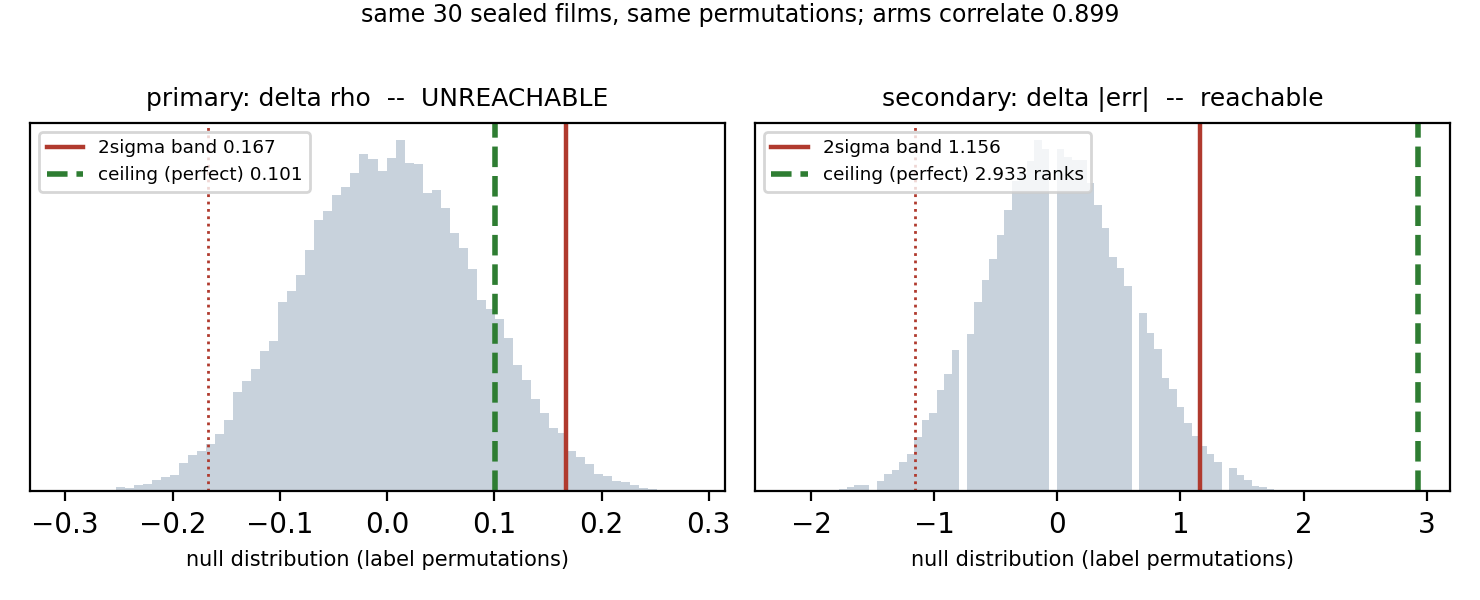
\includegraphics[width=\linewidth]{figs/bandceiling.png}
\caption{같은 30편, 같은 순열, 같은 귀무분포. 왼쪽 1차($\Delta\rho$):
초록 파선(완벽 예측)이 빨강 실선(밴드) \emph{안쪽}에 있다 --- 어떤
라벨로도 못 넘는다. 오른쪽 2차($\Delta|\text{err}|$): 같은 완벽
예측이 밴드 밖 $5.07\sigma$다. 전부 산출물에서 계산했다.}
\end{figure}

상관이 높은 두 예측을 비교할 때 상관계수의 \emph{차}는 천장이
눌린다. $\rho$가 $[-1,1]$에 갇혀 있으니 한쪽이 완벽해지면 다른
쪽도 따라 올라간다. 두 팔이 닮을수록 --- 즉 실험이 잘 통제될수록
--- 천장이 낮아지는 통계다. 짝 설계의 미덕이 통계의 결함으로
뒤집힌다.

\emph{정정판 부기.} 초판은 이 절을 \emph{``밴드를 잘못 고른 것이
아니라 통계를 잘못 골랐다''}로 닫았다. 절반만 맞다. 통계를 바꿔도
착지 예상 구간의 검정력은 5\%에서 8\%로 갈 뿐이다. 합성으로 $m$을
키워 보면 $m{=}120$에서 7\%, $m{=}500$에서 15\%, $m{=}2000$에서
48\%다 --- \textbf{이 짝 설계로 한 열을 전향 검증하는 길은 30편에
없다.}

\section{고친 것과, 고치지 않은 것}

편별 짝 통계로 바꿨다:
$\Delta|\text{err}| = \overline{|r_{\text{대조}}-r_{\text{라벨}}|}
- \overline{|r_{\text{국적}}-r_{\text{라벨}}|}$.
같은 순열에서 밴드 $1.1612$, 완벽 예측 $2.9333$ --- $5.07\sigma$.
천장이 상관에 눌리지 않는다.

\textbf{그런데 이건 골대 이동처럼 보인다.} 방어를 적어 둔다.
(1)~첫 봉인작 개봉이 이틀 뒤이고 \emph{라벨은 아직 존재하지 않는다}.
(2)~기존 1차 규칙은 한 글자도 안 고쳤고 9월에 그대로 계산 $\cdot$
보고된다. (3)~2차의 밴드 $\cdot$ $\tau$ $\cdot$ 갈래 넷을 지금 전부
얼렸다 --- 수확일에 고를 것이 없다. (4)~둘 다 보고한다.
(5)~무엇보다 2차를 고른 근거가 \textbf{라벨과 무관한 사실}
(두 팔의 상관 $0.899$)이다. 라벨을 한 톨도 안 보고 내린 결정이라는
것이 이 방어의 전부이고, 그래서 개봉 전에 해야만 했다.

고치지 않은 것도 적는다. 동결물의 국적 코드는 마스크 밖 채움값이
$0.5$인데 3범주에서 그 값은 \emph{미국}의 코드와 같다. 봉인 30편 중
4편이 그렇게 코딩됐다. 알려진 결함이고 \textbf{그대로 둔다} ---
라벨 전에 얼린 것을 라벨 전이라도 고치면 동결의 뜻이 없다. 대신
9월에 판정을 읽을 때 함께 읽으라고 사이드카에 적었다.

\section{교훈}

\textbf{예측을 얼린다는 것은 셋을 얼린다는 뜻이다} --- 예측, 채점기,
그리고 판정에 쓰는 모든 수. 셋 중 하나라도 라벨이 생긴 뒤에
만들어지면 그 자리에 재량이 들어간다. 나는 첫째만 얼려 놓고 셋 다
얼렸다고 적었다.

그리고 사전등록 체크리스트에 한 줄이 늘었다. 초판은 그 줄을
\emph{``완벽 예측이 밴드를 넘나?''}로 썼는데 \textbf{그것도
틀렸다} --- 정정판이 얼린 2차 통계는 그 검사를 $5.07\sigma$로
\emph{통과하면서} 검정력이 5\%였다. 필요조건을 충분조건 자리에
앉힌 것이다. 옳은 줄은 이렇다.

\begin{quote}
\textbf{사전등록한 관심 효과 크기가 밴드를 넘나 --- 그 크기에서
검정력이 몇 \%인가.} 그리고 \textbf{음성이 나오면 그것을 어떻게
읽을지}를 라벨이 생기기 전에 적어라.
\end{quote}

문턱을 정할 때 우리는 잡음의 크기만 본다. 신호가 갈 수 있는 가장
먼 곳도, \emph{실제로 기대하는 곳에서의 힘}도 함께 봐야 한다.
그 방이 없으면 두 달을 기다려 얻는 것은 답이 아니라 침묵이고,
침묵을 음성으로 읽는 순간 우리는 없는 증거를 만들어낸다.

이 논문이 두 번 틀린 방식이 같다. 초판은 천장을 재고
``불가능''이라 썼고, 그 초판의 전 사이클은 $+0.0168$을 보고
``전이가 눌렀다''고 썼다. \textbf{둘 다 잰 것에서 안 잰 것으로
건너뛴 문장이다.} 이 실험실의 만성병은 측정이 아니라 그 다음
문장에 있다.

\end{document}
